%\subsection{Simulation results}


%\emph{Dynamic demand.} Whey jobs are heterogeneous, demand is dynamic. We use simulator to evaluate the performance for demand detection and reallocation.
%\todo{present the dynamic demand case: what traces we use or what random distribution we are based on.}

\subsubsection{Simulation results}
\label{sec:large-sim}

%\todo{introduce other parameters in evaluation if any.}

%\paragraph{Average completion time.}
Figure \ref{fig:sim_large_scale} shows our simulation results. With a larger scale and more jobs, \name ($\alpha = 0.1$) consistently outperforms \DRFFIFO, \DRFSJF, \ESRP, and \DRFExt even more, reducing the completion time by 95\%, 84\%, 88\%, and 53\%, respectively.
Impressively, \name is not far (30\%) from \SRPT that only minimizes the average completion time without considering fairness, and with preemption allowed. 
When we focus on the longest 1\% jobs, \name has even larger improvements and beats \SRPT. This is not surprising because \SRPT prioritizes shorter jobs. 

%\begin{figure}[H]
%	\centering
%	{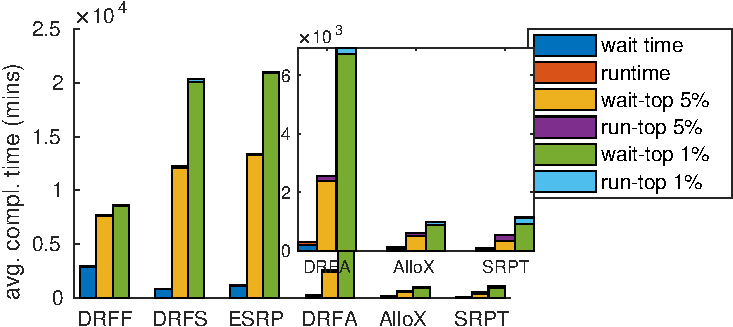
\includegraphics[width=1\linewidth]{figs/avgCmplt_m1}}    
%	\caption{[Simulation] AlloX outperforms others and is not far from the impractical SRPT in large-scale simulations. \todo{update the text accordingly.}}
%	\label{fig:sim_large_scale}
%\end{figure}

\begin{figure}[h]
	\centering
	\subfloat[all jobs]{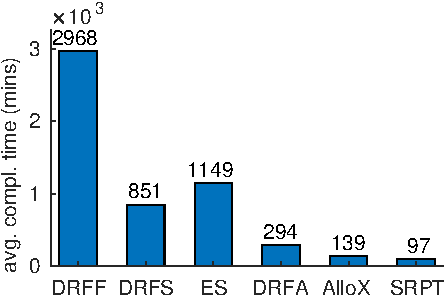
\includegraphics[width=0.47\linewidth]{figs/avgCmplt}}
	\subfloat[1\% longest jobs]{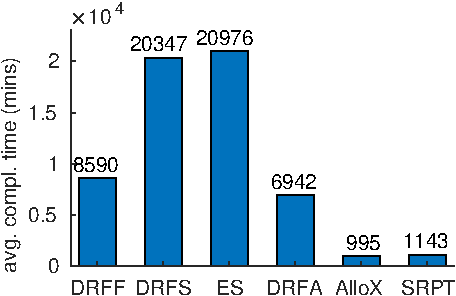
\includegraphics[width=0.47\linewidth]{figs/avgCmplt_99}}    
	\caption{[Simulation] AlloX outperforms others and is not far from the impractical SRPT in large-scale simulations.}
	\label{fig:sim_large_scale}
\end{figure}



%\paragraph{Performance overtime} 
%Scheduling jobs to minimize the average completion time may cause large jobs suffering from starvation.
%The error bars in Figure \ref{fig:sim_large_scale} show the average completion times of the top 5\% and 1\% of jobs. 
%Since \DRFSJF, \ESRP, \DRFExt, and \SRPT based on shortest job first schedules the long jobs last, the long-jobs can be starved.
%When there are many queued up jobs like \DRFSJF, the starvation is much more significant. \zhenhua{Why many queued up jobs in \DRFSJF?}
%\new{ \DRFSJF has much longer waiting time than \ESRP because it cannot handle the incoming load that results in more queued up jobs over time.
%}
%\todo{The starvation in SRPT is not noticeable.}


%To provide more details regarding the comparison , we show the job arrivals and average JCT over the time horizon in Figure \ref{fig:perf_overtime}.
%If the average completion times are very high at some periods, there are unscheduled jobs hungry for resources. \zhenhua{Why? Can that be from larger job sizes during those periods or longer queues instead of starvation?}
%\zhenhua{The following description is not clear. Do spikes imply starvation?}
%Recall that \DRFFIFO has the worst performance, it does not have large spikes.
%It is because \DRFFIFO serves the jobs in the FIFO manner so the jobs do not suffer from starvation.
%\DRFSJF has significant spikes.
%Basically, it scarifies starvation for performance. 
%Similarly, \ESRP, \DRFExt, and \SRPT also have noticeable spikes due to starvation.
%In contrast, \name 's average completion time of is the smoothest over time.
%Meaning, \name suffers least from starvation.


\begin{figure}[h]
	\centering
	\hspace{-0.3in}{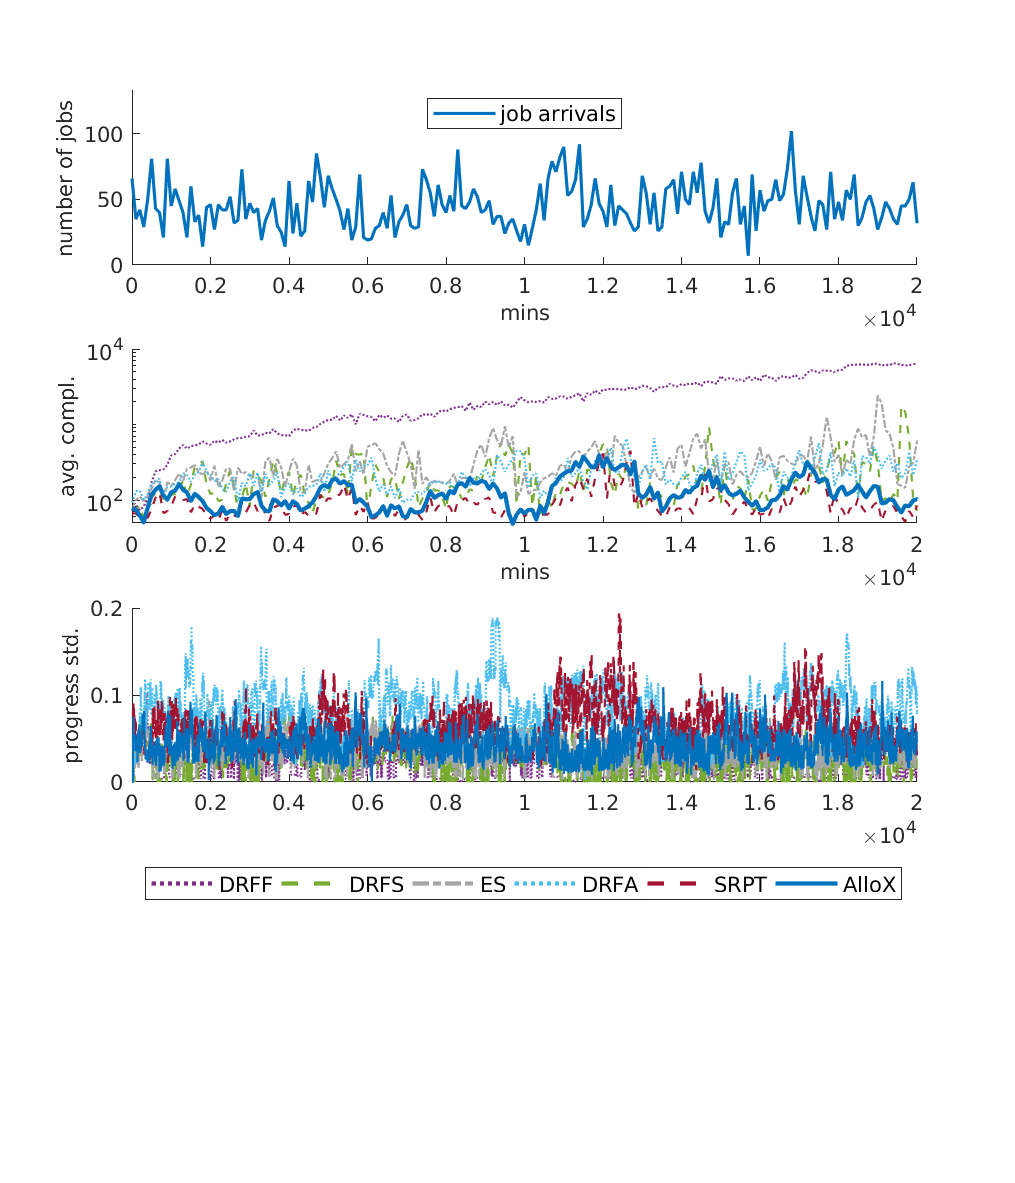
\includegraphics[width=1.1\linewidth]{figs/perf_overtime}}
	\vspace{-1in}
	\caption{[Simulation] \name consistently maintains the best performance over time, especially during the period with high arrival rates. \name also provides consistently small disparity across users' progress.}
	\label{fig:perf_overtime}
\end{figure}

To provide more details regarding the comparison, we show the job arrivals, average job completion time, and the standard deviation of progresses across users over time in Figure \ref{fig:perf_overtime}.
The average completion times of \name and \SRPT are consistently better over time compared to other baselines. Note the completion time is shown on a logarithmic scale.
When the arrival rates are high, the completion time of other baselines are much higher than that of \name. Not surprisingly, \DRFFIFO cannot process the jobs fast enough so queues build up. 
This highlights by effective scheduling and configuration selection, \name processes jobs faster and therefore allows for high arrival rates. %The large spike around the end is because some jobs running on CPUs finally finish, and artificially increases the average job completion time during this period. 

The figure also shows the disparity across users' progress over time. In this case, \SRPT and \DRFExt are much worse than \name, while DRFF, DRFS, and ES are a little better than \name (all users progress at similar, but much slower rates compared to \name). 
While the disparity in \SRPT is intuitive, \DRFExt fails to provide fairness because it ignores the different speedups of users, and instead use some averaged value to allocate resources. 

Overall, \name provides near optimal performance (similar to \SRPT) and maintains good fairness over time. 

\paragraph{Starvation}

In the extreme case, some users starve under schedulers like \SRPT. 
Figure \ref{fig:job_completed} shows the number of completed jobs of the user with longer jobs than others.
As expected, \SRPT performs the worst with most jobs unfinished.
In contrast, \name provides the best progress of this user because it maintains fairness similar to other baselines and is more effective. 


\begin{figure}[h]
	\centering
	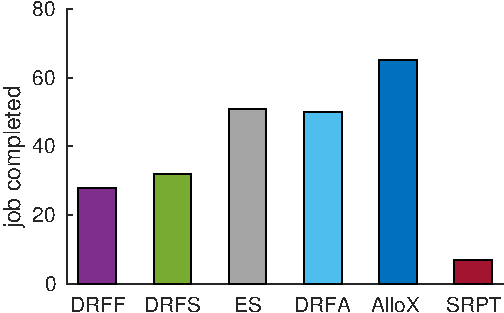
\includegraphics[width=0.7\linewidth]{figs/job_completed}  
	\caption{[Simulation] \name provides the best progress for users with longer jobs, and prevents starvation.}
	\label{fig:job_completed}
\end{figure}

\paragraph{Performance and fairness trade-offs}
\label{sec:tradeoffs}

Figure \ref{fig:fairness_alpha} shows the trade-offs between performance (average completion time) and fairness. 
We vary the parameter $\alpha$ from 0.1 to 1 (smaller means fairer) and compare the performance with \ESRP and \SRPT.
%Small $\alpha$ is better in terms of fairness.
This shows with larger $\alpha$, \name approaches \SRPT in performance. The small gap (9\%) between \name and \SRPT when $\alpha=1$ is due to the fact \SRPT is preemptive at no cost while \name does not allow preemption. 
However, the unfairness in terms of standard deviation of users' progress also increases with larger $\alpha$. Normally, a small $\alpha$ around 0.2 is good at providing large performance improvements at little cost of fairness. 
In practice, a system operator can pick the tradeoff according to her situation. 



%When $\alpha$ is large, \name has more queued jobs for scheduling so it performs better.
%Interestingly, it can reach closely to the performance of unrealistic \SRPT (2.2\%).


%We use Jain's fairness index (JFI) to measure the fairness.
%For fair comparison, we use resource usage as input for JFI for \DRFFIFO, \DRFSJF, \ESRP, and \DRFExt.
%Meanwhile, we use fairness cores as the input for \name and \SRPT.
%\SRPT is the best in terms of average completion time but worst in fairness.
%When we change $\alpha$, \name closes the performance gap with \SRPT.
%Meaning, \name can sacrifice fairness to gain performance.


\begin{figure}[h]
	\centering
	\subfloat[Performance]{{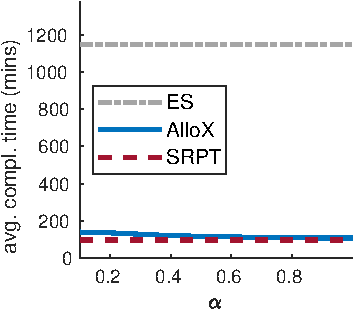
\includegraphics[width=0.47\linewidth]{figs/fairness_alpha}}}
	\hspace{0.05in}
    \subfloat[Fairness]{{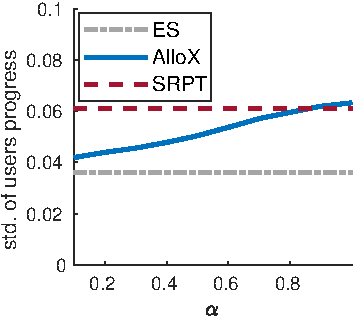
\includegraphics[width=0.47\linewidth]{figs/fairness_std_alpha}}}
	\caption{[Simulation] Performance and fairness trade-off. A larger $\alpha$ helps \name approach \SRPT at the cost of worse fairness. }
	\label{fig:fairness_alpha}
\end{figure}

\subsection{Sensitivity Analysis}
\label{sec:sensitivity}

\subsubsection{Estimation errors}
\label{sec:estimation_err}

%Estimation errors are unavoidable.
Figure \ref{fig:analysis_err} evaluates the impacts of mis-estimations on the performance, where we vary the standard deviation of errors from 0 to 60\%.
Even though \DRFFIFO does not need the estimation, its performance is too bad so we compare \name with a stronger baseline \ESRP. %we compare the average completion time of \name to  \DRFFIFO 's.
Even with large estimation errors, \name still provides large improvements that are similar to \SRPT. 
%When the errors are small (under 20\%), the improvements are unchanged.
%When the errors are large (up to 43\%), \name is better than \DRFFIFO.
This highlights the value of incorporating (even noisy) estimation from our estimator. 

\begin{figure}[h]
	\centering
	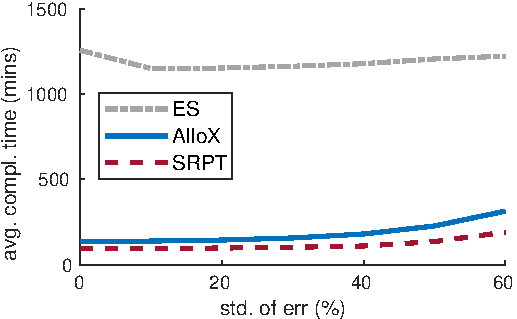
\includegraphics[width=0.9\linewidth]{figs/analysis_err}
	\caption{[Simulation]  \name is robust to the estimation errors.}%(\DRFSJF is better with large errors because they can utilize more CPUs.) \todo{update the text accordingly.}}
	\label{fig:analysis_err}
\end{figure}

\subsubsection{Profiling overhead}
\label{sec:overhead}

Estimations require running profiling jobs with some overhead. Running a longer sample of a job provides better estimations with larger overhead. 
%The scales of estimation overheads may vary in practice.
Figure \ref{fig:analysis_overhead} evaluates the impacts of profiling overheads on performance. Recall in our experiments have profiling overheads at 3\%.
As \DRFFIFO does not require estimation, its performance is unchanged.% we compare the performance of \name with \DRFFIFO.
With large overheads, the performance of all other solutions including \name and \SRPT degrades. 
However, \name provides consistent, significant improvements compared to other baselines. 
%When the overheads are small (under ??\%), the performance improvement are significant.
In practice, for long and iterative machine learning jobs, it is reasonable to use small sampling jobs. 
We can also obtain the runtime estimation from users \cite{tetrisched, choosy}, which may lead to further improvements.

\begin{figure}[h]
	\centering	
	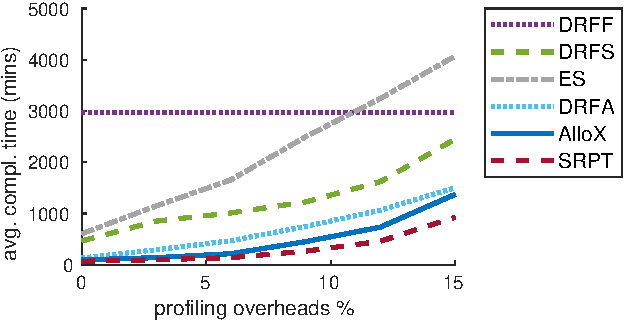
\includegraphics[width=0.9\linewidth]{figs/analysis_overhead_ext}
	\caption{[Simulation] Impacts of profiling overheads.}% must be small to have the small impacts on performance. Fortunately, sampling jobs can be much smaller than the full jobs as in our experiments. \todo{update the text accordingly.}}
	\label{fig:analysis_overhead}
\end{figure}

\subsubsection{Sensitivity to \name job subset size}
\label{sec:N_max}

Figure \ref{fig:analysis_N_max} shows the performance degradation of \name with smaller numbers of jobs used in the scheduling algorithm. There may be up to 200 jobs available for scheduling. As the figure shows, with a larger capacity of the system, more jobs should be included, but picking a small number already realizes most of the improvements. This allows \name to run at a much faster speed in practice. 
% We also have different capacity sizes.
% The maximum size of queued jobs of a user overtime is 97 (for capacity=20).
% The number of queued jobs linearly increases with the capacity.
% \name quickly converges at a small subset size that allows \name to overcome the computational bottleneck.

\begin{figure}[H]
	\centering
	{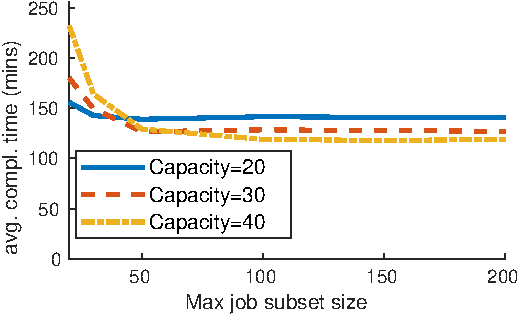
\includegraphics[width=0.9\linewidth]{figs/analysis_N_max_ext}}
	\caption{[Simulation] \name achieves most improvements by considering a small subset of available jobs. }
	\label{fig:analysis_N_max}
\end{figure}